\documentclass[12pt,a4paper,titlepage]{article}
\usepackage{graphicx}
\usepackage{graphics}
\usepackage{epsfig}
\usepackage{amsmath}
\usepackage{amssymb}
\usepackage{amsthm}
\usepackage{booktabs}
\usepackage{stmaryrd}
\usepackage{url}
\usepackage{longtable}
\usepackage[figuresright]{rotating}
\usepackage[utf8]{inputenc}
\usepackage[T1]{fontenc}
\usepackage[polish]{babel}
\usepackage{geometry}
\usepackage{pslatex}
\usepackage{ulem}
\usepackage{lipsum}
\usepackage{listings}
\usepackage{url}
\usepackage{Here}
\usepackage{color}
\usepackage[ruled,vlined,linesnumbered]{algorithm2e}
\selectlanguage{polish}
\definecolor{szary}{gray}{0.6}
\setlength{\textwidth}{400pt}
\lstset{numbers=left, numberstyle=\tiny, basicstyle=\scriptsize\ttfamily, breaklines=true, captionpos=b, tabsize=2}

\makeindex

\title{Faktoryzacja iloczynu kartezjańskiego grafów }
\date{30.06.2018}
\author{Andrzej Kawula \\ Promotor: dr Monika Pilśniak}

\begin{document}
\maketitle
\tableofcontents
\newpage
\section{Wprowadzenie}
\section{Wstęp}
\subsection{Informacje wstępne}
Produktem kartezjańskim $G_1 \square G_2 $ grafów $G_1 = (V_1 , E_1 ) $ i $ G_2 =(V_2 , E_2 ) $ nazywamy graf $G = (V, E)$, którego zbiorem wierzchołków jest iloczyn kartezjański wierzchołków grafów $G_1$ i $G_2$ $(V=V_1 \times V_2 )$, natomiast wierzchołki $(x_1, y_1)$ oraz $(x_2, y_2)$ są połączone w grafie $G$ jeżeli $x_1 = x_2$ oraz $y_1 y_2 \in E_2 $ lub $x_1 x_2 \in E_1 $ oraz $y_1 = y_2 $.\\
Iloczyn kartezjański grafów jest działaniem łącznym, przemiennym, z dokładnością do izomorfizu, elementem neutralym działania jest graf $K_1$.\\
Z łączności działania możemy zapisać $G_1 \square G_2 \square ... \square G_k = G$ gdzie $G$ jest produktem kartezjańskim grafów $G_1, G_2, ... , G_k$, a nastepnie poetykietować wierzchołki grafu G $k$-elementową listą $(v_1, v_2 , ... v_k )$ gdzie $v_i \in V(G_i)$ dla $1 \leqslant i \leqslant k $. Jeżeli $v$ etykietowny jest przez listę $(v_1, v_2 , ... v_k )$, można zdefiniować rzutowanie $p_i : V \rightarrow V_i $ dla $1 \leqslant i \leqslant k $, które dane jest wzorem $p_i (v) = v_i $, gdzie $v_i$ jest i-tym elemetem listy etykietującej wierzchołek $v$. Wierzchołek $v_i $ ten będzie i-tą współrzędną wierzchołka $v$.  \\
Jeżeli w grafie $G$ dany jest wierzchołek $v$ i rozważymy wierzchołki, które różnią się od wierzchołka $v$ tylko na i-tej pozycji, to podgraf indukownay przez te wierzchołki utowrzy graf izomorficzny  z grafem $G_i$. Podgraf ten będzie nazywany i-tą warsttwą $G_i$ przechodzącą przez wierzchołek $v$ a jego oznaczazeneim będzie $G_i ^v$.\\
Niech $v_0$ będzie wyróżnionym wierzchołkiem w grafie $G$. Warstwy przechodzące przez $v_0$ nazywamy warstwami jednostkowymi. Wierzchołek $v_0$ należy do każdej warstwy jednostkowej, natomiast zbiory $V(G_i ^{v_0}) \setminus \{v_0\}$ są parami rozłączne dla $1 \leqslant i \leqslant k $.
\\
Rysunek będzie zmieniony \\
\begin{figure}
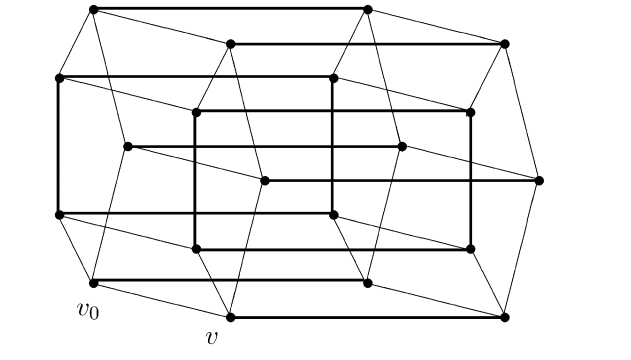
\includegraphics{rys1.png}
\end{figure}
\\
\subsection{Kolorowanie produktu iloczynu kartezjańskiego grafów}
Niech dane będą dwa połączone wierzchołki $u$ oraz $v$ w grafie G. Analizująć współrzędne tych wierzchołków, łatwo można stwierdzić że różnią się one dokładne na jednej pozycji. Niech $i$ oznacza tę pozycję. Wtedy krawędź $uv$ należy do $G_i^v$. Krawędzi $uv$  otrzymuje kolor $i$ czyli $c(uv) = i$, gdzie $c$ jest kolorwaniem własciwym produktu kartezjańskiego. Podsumowując: funkcja $c: E(G) \rightarrow {1,2,...,k}$ jest kolorowaniem własciwym produktu iloczynu kartezjańskiego jeżeli $c(uv) = i $ wtedy i tylko wtedy gdy współrzędne wierzchołków $u$ oraz $v$ różnią się na i-tej pozycji.\\
Każda krawędź należy dokładnie do jednej warstwy. Rozważając podgraf grafu $G$ skaładający się z krawędzi koloru $i$ to każda spójna składowa tego podgrafu będzie oddzielną i-tą warstwą grafu $G$.
\subsection{Lemat o kwadracie}
Niech graf $G$ posiada własciwe pokolorowanie produktu kartezjańskiego. Dane sa dwie połączone krawędzie $e$ i $f$ różnych kolorów. Wówczas istieje dokładnie jeden kwadrat bez przekątnych (graf $C_4$) zawierający $e$ oraz $f$.\\
\textit{Dowód:}\\
Na początku rozważmy nastepujący fakt. Każdy trójkąt w grafie $G$ jest pomalowany na ten sam kolor. Wynika to z tego, że dwa pierwsze wierzchołki różnią się na pozcyji i-tej, natomiast jeżeli wspólrzędne trzeciego wierzchołka różniły by się na pozycji $j$-tej która jest różna od $i$ w porównaniu z pierwszym wierzchołkiem i jego współrzędnymi, nie było by możliwosci aby drugi i trzeci wierzchołek byłby by ze sobą połączone, ponieważ ich współrzędne różniły by się na dwóch pozycjach.\\
Na podstawie powyższego stwierdzenia stwierdzamy, że każdy kwadrat zawierający co najmniej jedną przekątną jest tego samego koloru.\\
Teraz własciwy dowodu lematu. Dane są następujące oznaczenia:\\
$(v_0 , v_1, ... ,v_i, ..., v_j,...,v_k )$  współrzędne wspólnego wierzchołka $v$ krawędzi $e$ oraz $f$\\
$(v_0 , v_1, ... ,v'_i, ..., v_j,...,v_k )$ współrzędne wierzchołka $v_e$ który jest drugim końcem krawędzi $e$\\
$(v_0 , v_1, ... ,v_i, ..., v'_j,...,v_k )$ współrzędnymi wierzchołka $v_f$ który jest drugim końcem krawędzi $f$\\
$v'$ wierzchołek o współrzędnych $(v_0 , v_1, ... ,v_i', ..., v'_j,...,v_k )$\\ 
Łatwo stwierdzić, że wierzchołek $v'$ jest połączony z wierzchołkiem $v_e$ ponieważ ich współrzędne różnią się tylko na pozycji $j$ oraz w grafie $G_j$ istnieje krawędź $v_j v'_j$ ponieważ w grafie $G$ isnieje krawęź $f$. Analogicznie stwierdzamy istnienie krawędzi $v'v_f$, co w połączeniu z faktem, że krawędzie $e$ oraz $f$ są różnego koloru i rozważaniom na temat kwadratów z przekątnymi daje nam tezę lematu. Co więcej na podstawie powyższego rozumowania, można wnioskowaćy że przeciwległe krawędzie w kwadracie mają ten sam kolor, niezależnie czy kwadrat posiada przekątne czy też nie.
\subsection{Lemat o izomorfizmie}
Niech $G=(V, E)$ będzie spójnym grafem, natomiast $E_1 , E_2 , ... , E_k$ podziałem zbioru krawędzi. Niech każda spójna składowa $(V, \cup_{j \neq i}E_j)$ ma dokłdnie jeden punkt współny z każdą spóją skłądową $(V, E_i)$ oraz krawędzie między dwoma składowymi $(V, E_i)$ wyznaczają izomorfizm między tymi składowymi (jeżeli takie krawędzie istnieją). Wtedy:\\
$G=\Pi G_i $ \\
gdzie $G_i $ jest dowolną, spójną składową $(V, E_i)$.\\
\textit{Dowód:}\\
Tutaj chyba dowód indukcyjny ze względy na k, do sprawdzenia. 
\subsection{Lemat o udoskonaleniu faktoryzacji iloczynu kartezjańskiego}

\section{Algorytm Faktoryzacji}
\subsection{Faktoryzacja z dodatkowymi informacjami}
W tym podroździale przedstawimy algorytm kolorowania własciwego grafu względem iloczynu kartezjańskiego. Załóżmy, że mamy dane kolorywszystkich krawędzi wychodzących z pewnego wierzchołka $v_0$. Kolorowanie pozostałych krawędzi będzie odbywało się w kolejnosci przeszukiwania grafu w algorytmie BFS z wierzchołkiem początkowym $v_0$. \\
\\
\textit{Twierdzenie 3.1.1 Niech G=$G_1 \square G_2 \square ... \square G_k$ będzie grafem spójnym. Przypusćmy, że dane jest kolorawnie własciwe względem podanego rozkładu dla wszystkich krawędzi wychodzących z pewnego wierzchołka $v_0$. Wtedy  kolorowanie własciwe produktu kartezjańskiego może być uzyskane zgodnie z kolejnoscią algorytmu BFS o wierzchołku początkowym $v_0$. Złożonosć czasowa tego algorytmu to $\mathcal{O}$(mn), natomiast złożonosć pamięciowa $\mathcal{O}(n^2)$}.\\
\\
\textit{Dowód}\\
Jako dowód przedstawiony zostanie algorytm kolorwania krawędzi. W pierwszym kroku algorytmu dzielimy zbiór wierzchołków grafu $G$ na podzbiory $L_0 , L_1, L_2 , ..., L_r$ w taki sposób, że wierzchołek $v$ należy do zbioru $L_i$ wtedy i tylko wtedy gdy odległoćs wierzchołka $v$ od wierzchołka $v_0$ jest równa $i$. Zbiry te będziemy nazywać warstwami. Następnie dla każdego poziomu od 1 do r tworzymy trzy zbiory- krawędzie dolne, krawędzie poprzeczne oraz krawędzie górne. Definiowanie tych zbirów przebiega następująco. Rozważy poziom $i$, nastęnie dla wszystkich wierzchołków $v$ należących do zbioru $L_i$rozważamy krawędzie $vu$ incydentne z $v$. Wówczas jeżeli $u$ należy do $L_{i-1}$ to krawędź $vu$ będzie krawędzią dolną. Jeżeli $u$ należy do $L_i$ wówczas $uv$ będzie krawędzią poprzeczną, jeżeli natomiast $u$ należy do $L_{i+1}$ wówczas $uv$ będzie krawędzią górną wierzchołka warstwy $L_i$. Zauważmy, że krawędzie dolne warstwy $L_{i+1}$ to ten sam zbiór co krawędzie górne warstwy $L_{i}$ .\\
\\
Nasz algorytm rozpoczynamy od pokolorowania krawędzi poprzeczych $L_1$. Nie stanowi to problemy, ponieważ każdy trójkąt jest monochromatyczny. Tak więc każdej krawędzi $uv$ nadajemy kolor krawędzi $v_0 v$ czyli $c(uv):=c(v v_0 )=c(u v_0 )$.\\
\\
Następnie idnukcyjnie kolorujemy krawędzie dolne a następnie poprzeczne warstwy $L_{i+1}$ mając już pokolorowane krawędzie dolne i poprzeczne warstwy $L_i$. Nie ma potrzeby kolorowania krawędzi górnych warstwy $L_i$ ponieważ zbiór ten jest również zbiorem krawędzi dolnych warstwy $L_{i+1}$.\\
\\
Zaczynamy od krawędzi dolych. Przeglądamy wierzchołki należące do $L_{i+1}$ zgodnie z kolejnoscią wyznaczoną przez algorytm BFS. Niech dany będzie wierzchołek $u$ oraz krawędź $uv$. Ponieważ wierzchołek v należy do $L_i$, gdzie $i\geqslant 1$ to istnieje wierzchołek $w$ należący do $L_{i-1}$ incydentny z $v$. Rozważmy dwa przypadki:
\begin{enumerate}
\item Nie istnieje wspólny sąsiad wierzchołków $u$ oraz $w$ różny od $v$. Wówczas nie istnieje kwadrat zawierający wierzchołki $u$ oraz $w$ a co za tym idzie kolory krawędzi $uv$ oraz $vw$ są te same czyli $c(uv):=c(vw)$.
\item Istnieje wspólny sąsiad $x$ wierzchołków $u$ oraz $w$ różny od $v$. W tym przypadku $c(uv):=c(xw)$ oraz $c(ux):=c(vw)$. 
\end{enumerate}
Uzasadnienia w obydwu przypadkach wynikają z lematu o kwadracie (2.3).\\
Rozważmy teraz krawędzie poprzeczne warstwy $L_{i+1}$. W tym celu również przeglądamy wierzchołki należące do tej warstwy. Dla każdej krawędzi $uv$ należącej do krawędzi poprzecznych rozważaniej warstwy szukamy krawędzi dolnej $uw$ i podobnie jak dla krawędzi dolych szukamy wspólnego sąsiada wierzchołków $v$ oraz $w$. Jesli takowy wierzchołek $x$ instnieje wówczas $c(uv):=c(wx)$, jesli nie $c(uv):=c(uw)$.
\subsection{Nadawanie współrzędnych wierzchołkom}
\subsection{Etykietowanie produktu kartezjańskiego}
\subsection{Etykietowanie produktu w czasie liniowym}
\subsection{Sprawdzanie spójnosci kolorowanie właciwego produktu iloczynu kartezjańskiego}
\subsection{Opis algorytm faktoryzacji}
\section{Implementacja Algorytmu}
\subsection{Wprowadzenie}
\subsection{Dane wejsciowe}
\subsection{Opis pakietów i ważniejszych  klas}
\subsection{Opis algorytm faktoryzacji}
\end{document}